
    \begin{figure}[]
        \centering
		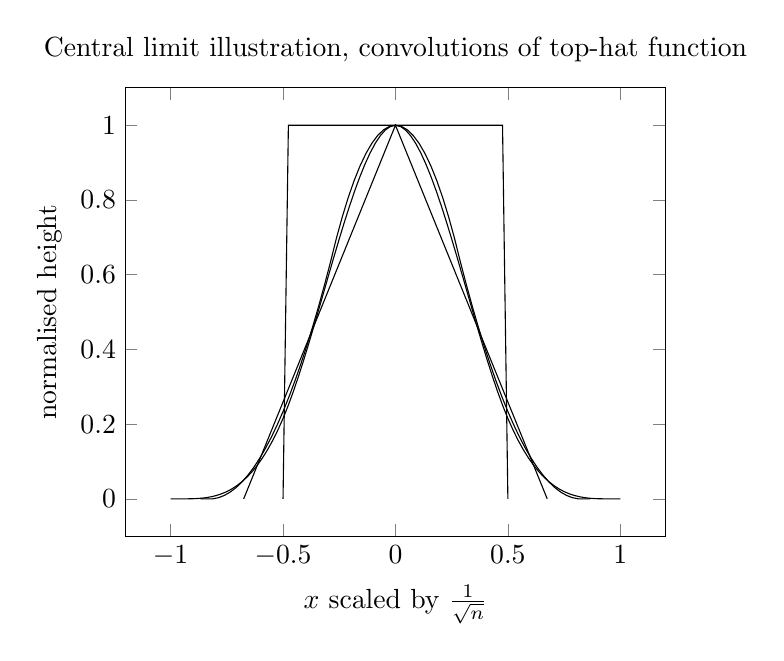
\begin{tikzpicture}
		\begin{axis}[
			title={Central limit illustration, convolutions of top-hat function},
			xlabel={$x$ scaled by $\frac{1}{\sqrt{n}}$},
			ylabel={normalised height},
		]
		\addplot[black] coordinates {
(-0.5, 0.0)(-0.47619047619047616, 1.0)(-0.4523809523809524, 1.0)(-0.4285714285714286, 1.0)(-0.40476190476190477, 1.0)(-0.38095238095238093, 1.0)(-0.35714285714285715, 1.0)(-0.33333333333333337, 1.0)(-0.30952380952380953, 1.0)(-0.2857142857142857, 1.0)(-0.2619047619047619, 1.0)(-0.23809523809523808, 1.0)(-0.2142857142857143, 1.0)(-0.19047619047619047, 1.0)(-0.16666666666666669, 1.0)(-0.14285714285714285, 1.0)(-0.11904761904761907, 1.0)(-0.09523809523809523, 1.0)(-0.07142857142857145, 1.0)(-0.047619047619047616, 1.0)(-0.023809523809523836, 1.0)(0.0, 1.0)(0.023809523809523836, 1.0)(0.04761904761904767, 1.0)(0.0714285714285714, 1.0)(0.09523809523809523, 1.0)(0.11904761904761907, 1.0)(0.1428571428571429, 1.0)(0.16666666666666663, 1.0)(0.19047619047619047, 1.0)(0.2142857142857143, 1.0)(0.23809523809523814, 1.0)(0.26190476190476186, 1.0)(0.2857142857142857, 1.0)(0.30952380952380953, 1.0)(0.33333333333333337, 1.0)(0.3571428571428571, 1.0)(0.38095238095238093, 1.0)(0.40476190476190477, 1.0)(0.4285714285714286, 1.0)(0.45238095238095233, 1.0)(0.47619047619047616, 1.0)(0.5, 0.0)
        }node[pos=0.91](endofplotsquare){} ;
		%\node [below,color={rgb:red,0;green,0;yellow,0}] at (endofplotsquare) {\footnotesize Our Bound};
		\addplot[black] coordinates {
(-0.6749655638598864, 0.0)(-0.6428243465332251, 0.047619047619047616)(-0.6106831292065639, 0.09523809523809523)(-0.5785419118799026, 0.14285714285714285)(-0.5464006945532413, 0.19047619047619047)(-0.51425947722658, 0.23809523809523808)(-0.48211825989991886, 0.2857142857142857)(-0.44997704257325755, 0.3333333333333333)(-0.41783582524659624, 0.38095238095238093)(-0.385694607919935, 0.42857142857142855)(-0.3535533905932738, 0.47619047619047616)(-0.3214121732666126, 0.5238095238095238)(-0.2892709559399513, 0.5714285714285714)(-0.25712973861329, 0.6190476190476191)(-0.2249885212866288, 0.6666666666666666)(-0.1928473039599675, 0.7142857142857143)(-0.1607060866333063, 0.7619047619047619)(-0.12856486930664499, 0.8095238095238095)(-0.09642365197998375, 0.8571428571428571)(-0.06428243465332253, 0.9047619047619048)(-0.032141217326661226, 0.9523809523809523)(0.0, 1.0)(0.032141217326661226, 0.9523809523809523)(0.06428243465332245, 0.9047619047619048)(0.09642365197998383, 0.8571428571428571)(0.12856486930664507, 0.8095238095238095)(0.1607060866333063, 0.7619047619047619)(0.1928473039599675, 0.7142857142857143)(0.22498852128662872, 0.6666666666666666)(0.25712973861328997, 0.6190476190476191)(0.28927095593995134, 0.5714285714285714)(0.3214121732666126, 0.5238095238095238)(0.3535533905932738, 0.47619047619047616)(0.385694607919935, 0.42857142857142855)(0.41783582524659624, 0.38095238095238093)(0.4499770425732576, 0.3333333333333333)(0.48211825989991886, 0.2857142857142857)(0.51425947722658, 0.23809523809523808)(0.5464006945532413, 0.19047619047619047)(0.5785419118799026, 0.14285714285714285)(0.6106831292065638, 0.09523809523809523)(0.6428243465332252, 0.047619047619047616)(0.6749655638598864, 0.0)
        }node[pos=0.5](endofplotsquare){} ;
		%\node [above,color={rgb:red,0;blue,0;yellow,0}, rotate=-45] at (endofplotsquare) {\footnotesize Entropy};
		\addplot[black] coordinates {
(-0.8660254037844386, 0.0)(-0.8397822097303648, 0.0)(-0.8135390156762908, 0.0)(-0.7872958216222169, 0.0030211480362537764)(-0.761052627568143, 0.00906344410876133)(-0.7348094335140691, 0.01812688821752266)(-0.7085662394599952, 0.030211480362537766)(-0.6823230454059213, 0.045317220543806644)(-0.6560798513518474, 0.0634441087613293)(-0.6298366572977735, 0.08459214501510574)(-0.6035934632436997, 0.10876132930513595)(-0.5773502691896258, 0.13595166163141995)(-0.5511070751355518, 0.1661631419939577)(-0.524863881081478, 0.19939577039274925)(-0.498620687027404, 0.23564954682779457)(-0.4723774929733301, 0.27492447129909364)(-0.4461342989192562, 0.31722054380664655)(-0.4198911048651824, 0.36253776435045315)(-0.3936479108111085, 0.4108761329305136)(-0.3674047167570345, 0.4622356495468278)(-0.34116152270296063, 0.5166163141993958)(-0.31491832864888675, 0.5740181268882175)(-0.2886751345948129, 0.6344410876132931)(-0.26243194054073893, 0.6978851963746223)(-0.23618874648666505, 0.7552870090634441)(-0.2099455524325912, 0.8066465256797583)(-0.1837023583785173, 0.851963746223565)(-0.15745916432444335, 0.8912386706948641)(-0.13121597027036946, 0.9244712990936556)(-0.1049727762162956, 0.9516616314199395)(-0.07872958216222171, 0.972809667673716)(-0.05248638810814775, 0.9879154078549849)(-0.026243194054073875, 0.9969788519637462)(0.0, 1.0)(0.026243194054073875, 0.9969788519637462)(0.05248638810814775, 0.9879154078549849)(0.07872958216222162, 0.972809667673716)(0.1049727762162955, 0.9516616314199395)(0.13121597027036955, 0.9244712990936556)(0.15745916432444343, 0.8912386706948641)(0.1837023583785173, 0.851963746223565)(0.2099455524325912, 0.8066465256797583)(0.23618874648666505, 0.7552870090634441)(0.26243194054073893, 0.6978851963746223)(0.2886751345948128, 0.6344410876132931)(0.3149183286488867, 0.5740181268882175)(0.34116152270296074, 0.5166163141993958)(0.3674047167570346, 0.4622356495468278)(0.3936479108111085, 0.4108761329305136)(0.4198911048651824, 0.36253776435045315)(0.4461342989192562, 0.31722054380664655)(0.4723774929733301, 0.27492447129909364)(0.498620687027404, 0.23564954682779457)(0.5248638810814779, 0.19939577039274925)(0.5511070751355519, 0.1661631419939577)(0.5773502691896258, 0.13595166163141995)(0.6035934632436997, 0.10876132930513595)(0.6298366572977735, 0.08459214501510574)(0.6560798513518474, 0.0634441087613293)(0.6823230454059213, 0.045317220543806644)(0.7085662394599952, 0.030211480362537766)(0.734809433514069, 0.01812688821752266)(0.7610526275681431, 0.00906344410876133)(0.787295821622217, 0.0030211480362537764)(0.8135390156762908, 0.0)(0.8397822097303648, 0.0)(0.8660254037844386, 0.0)
        }node[pos=0.7](endofplotsquare){} ;
		%\node [below,black, rotate=-45] at (endofplotsquare) {\footnotesize Efron};
		\addplot[black] coordinates {
(-1.0, 0.0)(-0.9772727272727273, 0.0)(-0.9545454545454546, 0.0)(-0.9318181818181819, 0.0)(-0.9090909090909091, 0.00016178611875101117)(-0.8863636363636364, 0.0006471444750040447)(-0.8636363636363636, 0.0016178611875101116)(-0.8409090909090909, 0.003235722375020223)(-0.8181818181818181, 0.0056625141562853904)(-0.7954545454545454, 0.009060022650056626)(-0.7727272727272727, 0.013590033975084938)(-0.75, 0.01941433425012134)(-0.7272727272727273, 0.026694709593916843)(-0.7045454545454546, 0.03559294612522246)(-0.6818181818181819, 0.046270829962789195)(-0.6590909090909092, 0.05889014722536806)(-0.6363636363636364, 0.07361268403171008)(-0.6136363636363636, 0.09060022650056625)(-0.5909090909090908, 0.11001456075068759)(-0.5681818181818181, 0.1320174729008251)(-0.5454545454545454, 0.15677074906972982)(-0.5227272727272727, 0.18443617537615273)(-0.5, 0.21517553793884484)(-0.4772727272727273, 0.2491506228765572)(-0.4545454545454546, 0.2865232163080408)(-0.43181818181818177, 0.32680795987704253)(-0.40909090909090906, 0.3695194952273095)(-0.38636363636363635, 0.41417246400258856)(-0.36363636363636365, 0.46028150784662675)(-0.34090909090909094, 0.507361268403171)(-0.31818181818181823, 0.5549263873159683)(-0.2954545454545454, 0.6024915062287656)(-0.2727272727272727, 0.6495712667853099)(-0.25, 0.695680310629348)(-0.2272727272727273, 0.7403332794046271)(-0.20454545454545459, 0.7830448147548941)(-0.18181818181818177, 0.8233295583238958)(-0.15909090909090906, 0.8607021517553793)(-0.13636363636363635, 0.8946772366930917)(-0.11363636363636365, 0.9247694547807798)(-0.09090909090909094, 0.9504934476621906)(-0.06818181818181823, 0.971363856981071)(-0.045454545454545414, 0.9868953243811681)(-0.022727272727272707, 0.9966024915062288)(0.0, 1.0)(0.022727272727272707, 0.9966024915062288)(0.045454545454545414, 0.9868953243811681)(0.06818181818181812, 0.971363856981071)(0.09090909090909083, 0.9504934476621906)(0.11363636363636354, 0.9247694547807798)(0.13636363636363646, 0.8946772366930917)(0.15909090909090917, 0.8607021517553793)(0.18181818181818188, 0.8233295583238958)(0.20454545454545459, 0.7830448147548941)(0.2272727272727273, 0.7403332794046271)(0.25, 0.695680310629348)(0.2727272727272727, 0.6495712667853099)(0.2954545454545454, 0.6024915062287656)(0.3181818181818181, 0.5549263873159683)(0.34090909090909083, 0.507361268403171)(0.36363636363636354, 0.46028150784662675)(0.38636363636363646, 0.41417246400258856)(0.40909090909090917, 0.3695194952273095)(0.4318181818181819, 0.32680795987704253)(0.4545454545454546, 0.2865232163080408)(0.4772727272727273, 0.2491506228765572)(0.5, 0.21517553793884484)(0.5227272727272727, 0.18443617537615273)(0.5454545454545454, 0.15677074906972982)(0.5681818181818181, 0.1320174729008251)(0.5909090909090908, 0.11001456075068759)(0.6136363636363635, 0.09060022650056625)(0.6363636363636365, 0.07361268403171008)(0.6590909090909092, 0.05889014722536806)(0.6818181818181819, 0.046270829962789195)(0.7045454545454546, 0.03559294612522246)(0.7272727272727273, 0.026694709593916843)(0.75, 0.01941433425012134)(0.7727272727272727, 0.013590033975084938)(0.7954545454545454, 0.009060022650056626)(0.8181818181818181, 0.0056625141562853904)(0.8409090909090908, 0.003235722375020223)(0.8636363636363635, 0.0016178611875101116)(0.8863636363636365, 0.0006471444750040447)(0.9090909090909092, 0.00016178611875101117)(0.9318181818181819, 0.0)(0.9545454545454546, 0.0)(0.9772727272727273, 0.0)(1.0, 0.0)
        }node[pos=0.7](endofplotsquare){} ;
		%\node [below,black, rotate=-45] at (endofplotsquare) {\footnotesize Efron};
		
		\end{axis}
		\end{tikzpicture}
		%\vspace{-18pt}
		\caption{self convolutions of the top hat function (ie. probability distribution of the uniform function) for $n=1,2,3,4$ shows rapid convergence to gaussian distribution}
		\label{fig:central_limit_theorem}
    \end{figure}
